\documentclass[UTF8, 10pt, a4paper, oneside]{ctexart}
\usepackage{amsmath}
\usepackage{amsthm}
\usepackage{amsfonts}
\usepackage{amssymb}
\usepackage{amstext}
\usepackage[version=4]{mhchem}
\usepackage{geometry}
\usepackage{changepage}
\usepackage{paralist}
\usepackage{graphicx}
\usepackage{extarrows}
\usepackage{xcolor}
\geometry{left=1.27cm, right=1.27cm, top=1.27cm, bottom=1.5cm}
\linespread{1.5}
\title{\vspace{-2em} 高考模拟卷 \vspace{-1em}}
\author{盛炯元 \quad 杨元谦}
\date{\textcolor{white}{\today}\vspace{-3em}}
\pagestyle{plain}

\newcommand{\blank}{ \underbar{\quad$\blacktriangle$\quad} }% 空格样式
\newcommand{\fs}[1]{{\fangsong #1}}% 使用仿宋
\newcommand{\hei}[1]{{\heiti #1}}
\newcommand{\circled}[1]{{\small{\textcircled{\tiny{#1}}}}}% 圈圈数字
\newcommand{\Romannumeral}[1]{\uppercase\expandafter{\romannumeral#1}}% 大写罗马数字
\newcommand{\chdots}{…\hspace{-0.15em}…}% 中文省略号调教

\theoremstyle{definition}
\newtheorem{exercise}{}

\theoremstyle{remark}
\newtheorem*{answer}{【答案】}
\newtheorem*{point}{【考点】}      % 考点&易错点
\newtheorem*{explanation}{【解析】}     %

\theoremstyle{plain}
\newtheorem*{note}{【注】}  %(可选)

\begin{document}
\maketitle
\begin{exercise}
    在硝化细菌中,不会发生的生命活动是\quad(\quad)
    \begin{center}
        \begin{inparaenum}[\qquad A. ]
            \item[\setcounter{enumi}{1}A. ] 核膜的消失与重建
            \item 核酸-蛋白质复合物的形成与消失
            \item 氧气的摄取
            \item ATP的合成与水解
        \end{inparaenum}
    \end{center}
    \begin{answer}
        A
    \end{answer}
    \begin{point}
        原核与真核细胞的差异、化能合成作用
    \end{point}
    \begin{explanation}
        原核生物是原核细胞,没有以核膜为界限的细胞核,不存在增殖时周期性的核膜消失与重建,A选项错误;在基因转录、复制时,会有RNA聚合酶或DNA聚合酶与DNA分子结合形成核酸-蛋白质复合物,B选项正确;在化能合成作用中,硝化细菌需要借助氧气氧化氨或亚硝酸盐,C选项正确;ATP作为能量货币,能量在各生化反应中流动伴随着ATP的合成与水解,D选项正确。
    \end{explanation}
\end{exercise}
\begin{exercise}
    蛋白质是结构和功能多样的生物大分子,下列叙述正确的是\quad(\quad)
    \begin{adjustwidth}{2em}{}
        \begin{asparaenum}[A. ]
            \item 二硫键的断裂不会改变蛋白质的空间结构
            \item 血浆里,人体三大供能物质中质量分数最大的是蛋白质
            \item 向蛋白质溶液中加入浓的硫酸铜溶液可使蛋白质发生盐析
            \item 利用基因工程可以“创造”出自然界中原先不存在的蛋白质
        \end{asparaenum}
    \end{adjustwidth}
    \begin{answer}
        B
    \end{answer}
    \begin{point}
        蛋白质空间结构、血液中糖脂蛋相对含量、盐析与变性、基因工程局限性
    \end{point}
    \begin{explanation}
        二硫键影响蛋白质的三、四级结构,进而影响其整体空间结构,A选项错误;血浆中水占91\%$\sim$92\%,蛋白质约占7\%\textsuperscript{\fs{[义务教育教科书·生物学七年级下册 P35]}},B选项正确;铜离子是重金属,会使蛋白质发生变性,而不是盐析,C选项错误;基因工程原则上只能生产自然界中已存在的蛋白质,D选项错误。
    \end{explanation}
\end{exercise}

\begin{exercise}
    在一定温度下,大田的某种植物绿色叶片的光合速率和呼吸速率的平均对光照强度的响应曲线如图所示。下列说法错误的是\quad(\quad)
    \begin{adjustwidth}{2em}{}\vspace{-3em}
        \begin{figure}[h!]
            \flushright
            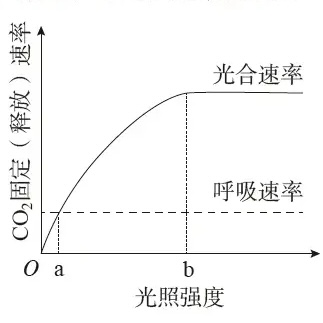
\includegraphics[width=0.3\textwidth]{assists/2-1.jpg}
        \end{figure}\vspace{-15em}
        \begin{asparaenum}[A. ]
            \item 生长于光照强度为a环境的植株生长最将因匮乏营养而死亡
            \item 光照强度从a逐渐增加到b时,该植物生长速率逐渐增大
            \item 光照强度小于b时,提高大田$\ce{CO2}$浓度,$\ce{CO2}$固定速率会增大
            \item 光照强度为b时,适当降低光反应速率,$\ce{CO2}$固定速率会降低
        \end{asparaenum}\vspace{0.5em}
    \end{adjustwidth}
    \begin{answer}
        C
    \end{answer}\vspace{0.25em}
    \begin{point}
        总光合速率、净光合速率\vspace{0.5em}
    \end{point}
    \begin{explanation}
        生长于光照强度为a环境的植株虽然其叶片的总光合速率与呼吸速率相等,但植株中总有无法进行光合作用的组织(如根、花、果实)消耗着贮存的有机物,A选项正确;光照强度小于b时,影响光合作用的主要因素为光照,提高大田$\ce{CO2}$浓度不一定h使$\ce{CO2}$固定速率增大,C选项错误。
    \end{explanation}
\end{exercise}

\begin{exercise}
    葡萄糖转运蛋白4(GLUT4)是一种存在于脂肪细胞中的蛋白质。在胰岛素的刺激下,GLUT4会从脂肪细胞内的囊泡膜上转移至细胞膜上,葡萄糖借助细胞膜上的GLUT4进入脂肪细胞。下列叙述错误的是 \quad(\quad)
    \begin{adjustwidth}{2em}{}
        \begin{asparaenum}[A. ]
            \item 脂肪细胞中GLUT4以氨基酸为原料,在核糖体中合成
            \item GLUT4转移至细胞膜所需要的能量主要来自于线粒体
            \item GLUT4每次转运葡萄糖时,其自身构象都会发生改变
            \item 当血糖浓度升高时,脂肪细胞膜上的GLUT4数量减少
        \end{asparaenum}
    \end{adjustwidth}
    \begin{answer}
        D
    \end{answer}
    \begin{point}
        蛋白质的生物合成、主动运输、胞间信息传递
    \end{point}
    \begin{explanation}
        当血糖浓度升高时,胰岛B细胞受刺激分泌更多胰岛素,促进更多GLUT4从脂肪细胞内的囊泡膜上转移至细胞膜上,故D选项错误。
    \end{explanation}
\end{exercise}

\begin{exercise}
    某研究团队测定了水分胁迫(不足或过多)下黄芩叶片的生理指标,结果如表所示。下列叙述正确的是\quad(\quad)
    \begin{figure}[h!]
        \centering
        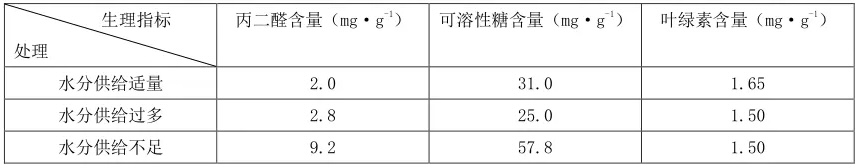
\includegraphics[width=0.8\textwidth]{assists/4-1.jpg}
    \end{figure}\vspace{-1em}

    (注:在胁迫状态下,细胞积累的活性氧会破坏膜的脂质分子,形成丙二醛)
    \begin{adjustwidth}{2em}{}
        \begin{asparaenum}[A. ]
            \item 氧自由基会攻击膜的组分蛋白质分子时,产物也是自由基,引发雪崩式反应
            \item 水分过多时,细胞膜完整性受损,控制物质进出的能力减弱
            \item 水分不足时,细胞内可溶性糖含量的变化导致水分流失增加
            \item 无论水分供给过多或不足,叶片内叶绿素含量相同,推测叶绿素的合成与水分供给无关
        \end{asparaenum}
    \end{adjustwidth}
    \begin{answer}
        B
    \end{answer}
    \begin{point}
        细胞衰老——自由基学说、数据分析
    \end{point}
    \begin{explanation}
        自由基攻击蛋白质分子会使蛋白质活性下降,但产物不是自由基,当自由基攻击磷脂时,产物才也是自由基,引发雪崩式反应,A选项错误;注意到水分过多时,细胞内可溶性糖含量显著降低,控制物质进出的能力减弱,B选项正确;水分不足时,胞内可溶性糖含量升高,渗透压升高,更不易流失水分,C选项错误;无论水分供给过多或不足,叶片内叶绿素含量都减少,叶绿素合成与水分供给有关,D选项错误。
    \end{explanation}
\end{exercise}
\begin{exercise}
    生菜是一种在保存和运输过程中易发生褐变的蔬菜。多酚氧化酶(PPO)在有氧条件下能催化酚类物质形成褐色的醌类物质,导致植物组织褐变。某团队研究生菜多酚氧化酶在不同条件下的特性,结果如图所示。下列叙述正确的是\quad(\quad)
    \begin{figure}[h!]
        \centering
        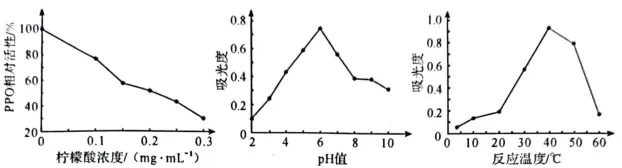
\includegraphics[width=0.8\textwidth]{assists/6-1.jpg}
    \end{figure}
    (注:吸光度大小与醌类物质含量成正相关)\vspace{-1em}
    \begin{adjustwidth}{2em}{}
        \begin{asparaenum}[A. ]
            \item 低氧环境可促进褐变发生
            \item 柠檬酸有抗氧化作用
            \item 保存和运输生菜的最适pH值为6
            \item 40$^\circ$C时PP0活性最高,适于生菜保存
        \end{asparaenum}
    \end{adjustwidth}
    \begin{answer}
        B
    \end{answer}
    \begin{point}
        数据分析
    \end{point}
    \begin{explanation}
        褐变的实质是氧化,故低氧环境能减缓褐变的发生,A选项错误;随着柠檬酸浓度上升,多酚氧化酶的活性下降,褐变(氧化)减缓,故柠檬酸有抗氧化作用,B选项正确;当pH为6时,吸光度最高,褐变(氧化)程度最高,不宜用于保存和运输,C选项错误;当反应温度为40$^\circ$C时,吸光度最高,褐变(氧化)程度最高,不宜用于保存和运输,D选项错误。
    \end{explanation}
\end{exercise}
\begin{exercise}
    生长于NaCl浓度稳定在100 mmol/L的液体培养基中的酵母菌,可通过离子通道吸收$\ce{Na+}$,但细胞质基质中$\ce{Na+}$浓度超过30 mmol/L时会导致酵母菌死亡。为避免细胞质基质中$\ce{Na+}$浓度过高,液泡膜上的蛋白N可将$\ce{Na+}$以主动运输的方式转运到液泡中,细胞膜上的蛋白W也可将$\ce{Na+}$排出细胞。下列叙述错误的是\quad(\quad)
    \begin{adjustwidth}{2em}{}
        \begin{asparaenum}[A. ]
            \item $\ce{Na+}$在液泡中的积累有利于酵母细胞吸水
            \item 蛋白N转运$\ce{Na+}$过程中自身构象会发生改变
            \item 通过蛋白W外排$\ce{Na+}$的的过程不需要细胞提供能量
            \item $\ce{Na+}$通过离子通道进入细胞时不需要与通道蛋白结合
        \end{asparaenum}
    \end{adjustwidth}
    \begin{answer}
        C
    \end{answer}
    \begin{point}
        主动运输、被动运输、渗透作用
    \end{point}
    \begin{explanation}
        生长在NaCl浓度稳定在100 mmol/L的液体培养基中,而细胞质基质中$\ce{Na+}$浓度超过30 mmol/L时会导致酵母菌死亡,可以推知通过蛋白W外排$\ce{Na+}$的的过程是逆浓度梯度的主动运输,需要细胞提供能量,C选项错误。
    \end{explanation}
\end{exercise}

\begin{exercise}
    有丝分裂过程中SMC3蛋白在着丝粒区大量富集。研究者通过构建玉米SMC3基因缺失突变体,观察野生型和突变体有丝分裂过程,部分结果如下图(A、B为同一时期,C、D为同一时期)。下列有关叙述正确的是\quad(\quad)
    \begin{figure}[h!]
        \flushright
        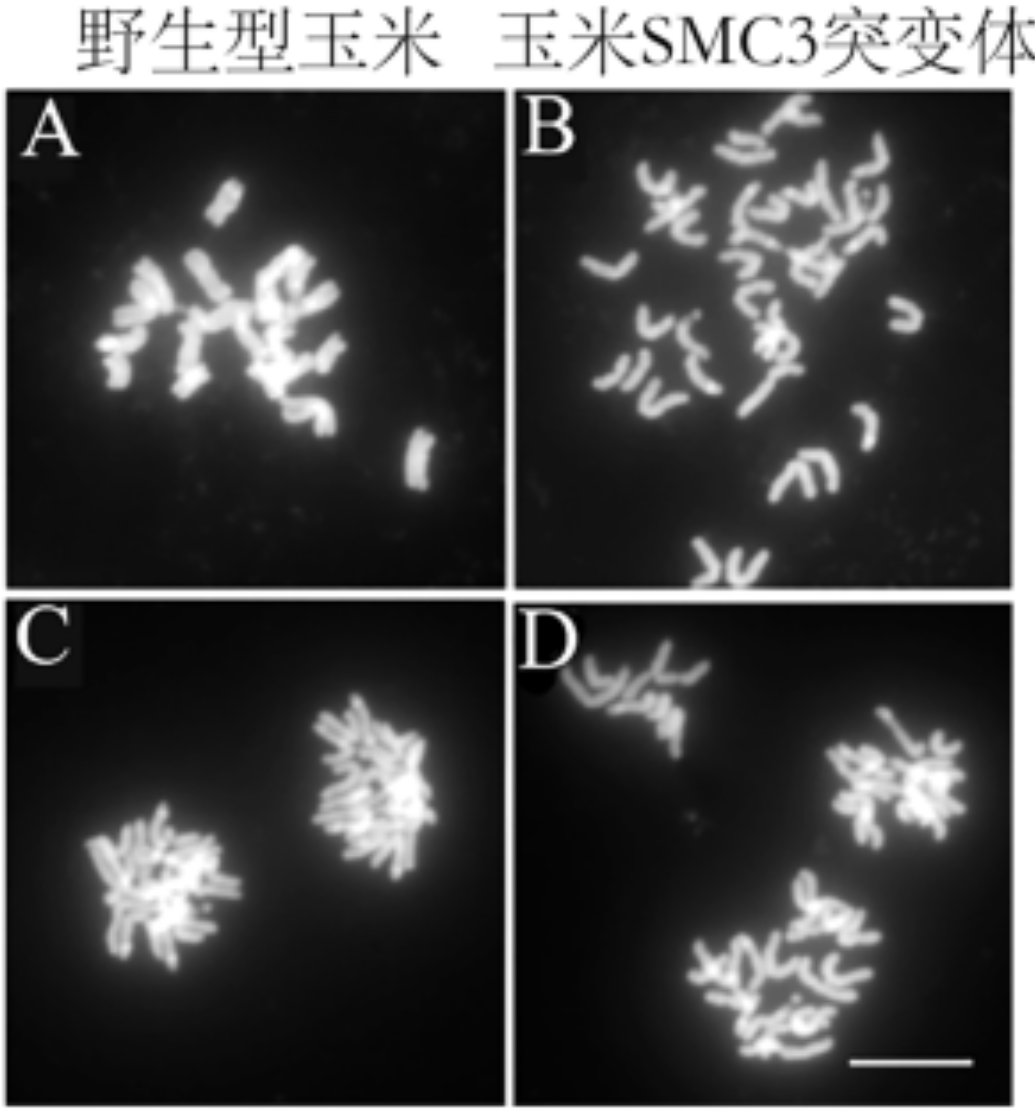
\includegraphics[width=0.25\textwidth]{assists/8-1.jpg}
    \end{figure}\vspace{-16em}
    \begin{adjustwidth}{2em}{}
        \begin{asparaenum}[A. ]
            \item 图B中染色体数目较图A多,推测SMC3突变体中染色体着丝粒易分裂
            \item 秋水仙素主要作用于图A所处时期的下个时期
            \item 图A、图C中的同源染色体对数和核DNA分子数都相同
            \item 野生型和突变体杂交后代,染色体数目一定异常
        \end{asparaenum}
    \end{adjustwidth}
    \begin{answer}
        A
    \end{answer}
    \begin{point}
        有丝分裂图像识读、染色体行为、秋水仙素作用
    \end{point}
    \begin{explanation}
        图A、B处于前期,图C、D处于后期。

        \noindent 图A下个时期是有丝分裂中期,而秋水仙素在有丝分裂后期生效,B选项错误;假设野\\生型玉米的染色体2N,则同源染色体:N(图A)、2N(图B),核DNA均为4N,C选项错误;题目中主要强调SMC3影响有丝分裂,可能不影响减数分裂,故D选项错误。
    \end{explanation}
\end{exercise}
\begin{exercise}
    淀粉类种子萌发形成幼苗离不开糖类等能源物质,也离不开水和无机盐。下列叙述正确的是\quad(\quad)
    \begin{adjustwidth}{2em}{}
        \begin{asparaenum}[A. ]
            \item 种子吸收的水与多糖等物质结合后,水仍具有溶解性
            \item 种子萌发过程中糖类含量逐渐下降,有机物种类不变
            \item 幼苗根细胞中的无机盐可参与细胞构建,水不参与
            \item 幼苗中的水可参与形成NADPH,也可参与形成NADH
        \end{asparaenum}
    \end{adjustwidth}
    \begin{answer}
        D
    \end{answer}
    \begin{point}
        结合水、种子的萌发
    \end{point}
    \begin{explanation}
        结合水失去了流动性和溶解性,成为生物体的构成部分,A选项错误;种子萌发过程中糖类含量逐渐下降,有机物种类增多,B选项错误;结合水是细胞结构的重要组成部分,也参与细胞的构建,C选项错误;幼苗进行光合作用时,光反应阶段中水光解产生的 $\ce{H^+}$ 和被叶绿体夺去的电子与 $\ce{NADP+}$ 结合生成 NADPH,幼苗进行有氧呼吸时,在第二阶段丙酮酸和水分解成 $\ce{CO2}$ 和 NADH,D选项正确。
    \end{explanation}
\end{exercise}
\begin{exercise}
    浆细胞合成抗体分子时,先合成的一段肽链(信号肽)与细胞质中的信号识别颗粒(SRP)结合,肽链合成暂时停止。待SRP与内质网上SRP受体结合后,核糖体附着到内质网膜上,将已合成的多肽链经SRP受体内的通道送入内质网腔,继续翻译直至完成整个多肽链的合成并分泌到细胞外。下列叙述正确的是\quad(\quad)
    \begin{adjustwidth}{2em}{}
        \begin{asparaenum}[A. ]
            \item SRP与信号肽的识别与结合具有特异性
            \item SRP受体缺陷的细胞无法合成多肽链
            \item 核糖体和内质网之间通过囊泡转移多肽链
            \item 生长激素和性激素均通过此途径合成并分泌
        \end{asparaenum}
    \end{adjustwidth}
    \begin{answer}
        A
    \end{answer}
    \begin{point}
        分泌蛋白的合成路径
    \end{point}
    \begin{explanation}
        即使SRP受体缺陷,浆细胞仍能合成信号肽这一多肽链(举反\([0-9]\)例),B选项错误;核糖体和内质网依赖于SRP与SRP受体的高亲和力结合,不依赖于囊泡,C选项错误;性激素是固醇,不是蛋白质,不通过上述路径合成或分泌,D选项错误。
    \end{explanation}
\end{exercise}

\begin{exercise}
    过氧化物酶体是存在于动植物细胞中的一种单层膜细胞器,可来源于线粒体和内质网分泌的囊泡的融合。该细胞器中主要含有氧化酶和过氧化氢酶类,氧化酶消耗氧气将底物氧化分解并产生过氧化氢,过氧化氢酶将过氧化氢分解为水和氧气。下列有关叙述错误的是\quad(\quad)
    \begin{adjustwidth}{2em}{}
        \begin{asparaenum}[A. ]
            \item 过氧化物酶体的形成体现了生物膜的流动性
            \item 过氧化物酶体在植物中可能参与光呼吸
            \item 过氧化物酶体在功能上与线粒体等典型需氧细胞器相似
            \item 过氧化物酶体属于细胞的生物膜系统
        \end{asparaenum}
    \end{adjustwidth}
    \begin{answer}
        C
    \end{answer}
    \begin{point}
        细胞器、阅读理解、生物膜系统、光呼吸
    \end{point}
    \begin{explanation}
        在强光下,植物光呼吸会产生过氧化物,过氧化物酶体可以分解过氧化物,避免组织损伤,故推测可能参与光呼吸,B选项正确;过氧化物酶体的主要功能是分解过氧化物,避免因过氧化物造成的组织损伤,其反应能量完全以热能散失,无法供能,而线粒体等经典需氧细胞器的主要功能是氧化分解有机物,利用长电子传递链将氧化放出的能量转移到ATP中供能,两者在功能上有较大差别,C选项错误。
    \end{explanation}
\end{exercise}

\begin{exercise}
    水淹时,玉米根细胞由于较长时间进行无氧呼吸导致能量供应不足,使液泡膜上的$\ce{H+}$转运减缓,引起细胞质基质内$\ce{H+}$积累,无氧呼吸产生的乳酸也使细胞质基质pH降低。pH降低至一定程度会引起细胞酸中毒。
    细胞可通过将无氧呼吸过程中的丙酮酸产乳酸途径转换为丙酮酸产酒精途径,延缓细胞酸中毒。下列说法正确的是\quad(\quad)
    \begin{adjustwidth}{2em}{}
        \begin{asparaenum}[A. ]
            \item 正常玉米根细胞液泡内pH高于细胞质基质
            \item 检测到水淹的玉米根有$\ce{CO2}$的产生不能判断是否有酒精生成
            \item 转换内丙酮酸产酒精途径时释放的ATP增多以缓解能量供应不足
            \item 转换为丙酮酸产酒精途径时消耗的[H]增多以缓解酸中毒
        \end{asparaenum}
    \end{adjustwidth}
    \begin{answer}
        B
    \end{answer}
    \begin{point}
        呼吸作用的应用、胞内物质运输
    \end{point}
    \begin{explanation}
        正常玉米根细胞液泡膜上的$\ce{H+}$转运蛋白是主动运输,逆浓度梯度,故正常正常玉米根细胞液泡内pH低于细胞质基质,A选项错误;有氧呼吸也释放$\ce{CO2}$,B选项正确;无论丙酮酸转换成什么,无氧呼吸第二步均不释放能量,不产生ATP,无法缓解能量供应不足,C选项错误;产酒精和产乳酸消耗的NADH相同,产酒精途径能缓解细胞酸中毒的原因是减少了乳酸这个“酸”的生成,D选项错误。
    \end{explanation}
\end{exercise}
\begin{exercise}
    为探究酵母菌的呼吸方式,可利用酵母菌,葡萄糖溶液等材料进行实验。下列关于该实验的叙述,正确的是\quad(\quad)
    \begin{adjustwidth}{2em}{}
        \begin{asparaenum}[A. ]
            \item 酵母菌用量和葡萄糖溶液浓度是本实验的自变量
            \item 酵母菌可利用的氧气量是本实验的无关变量
            \item 可选用酒精和$\ce{CO2}$生成量作为因变量的检测指标
            \item 不同方式的细胞呼吸消耗等量葡萄糖所释放的能量相等
        \end{asparaenum}
    \end{adjustwidth}
    \begin{answer}
        C
    \end{answer}
    \begin{point}
        细胞呼吸
    \end{point}
    \begin{explanation}
        酵母菌用量和葡萄糖溶液浓度是本实验的无关变量,酵母菌可利用的氧气量是本实验的自变量,A、B选项错误;1 mol葡萄糖经有氧呼吸可产生 6 mol $\ce{CO2}$,1 mol葡萄糖经无氧呼吸可产生 2 mol酒精和 2 mol $\ce{CO2}$,故可选用酒精和 $\ce{CO2}$ 生成量作为因变量的检测指标,C选项正确;消耗等量的葡萄糖,有氧呼吸释放的能量远多于无氧呼吸所释放的能量,D选项错误。
    \end{explanation}
\end{exercise}

\begin{exercise}
    部分厌氧菌缺乏处理氧自由基的酶,可进行不产氧光合作用,避免产生的氧自由基对自身造成伤害。如图表示绿硫细菌的光反应过程示意图,下列叙述正确的是\quad(\quad)
    \begin{figure}[h!]
        \centering
        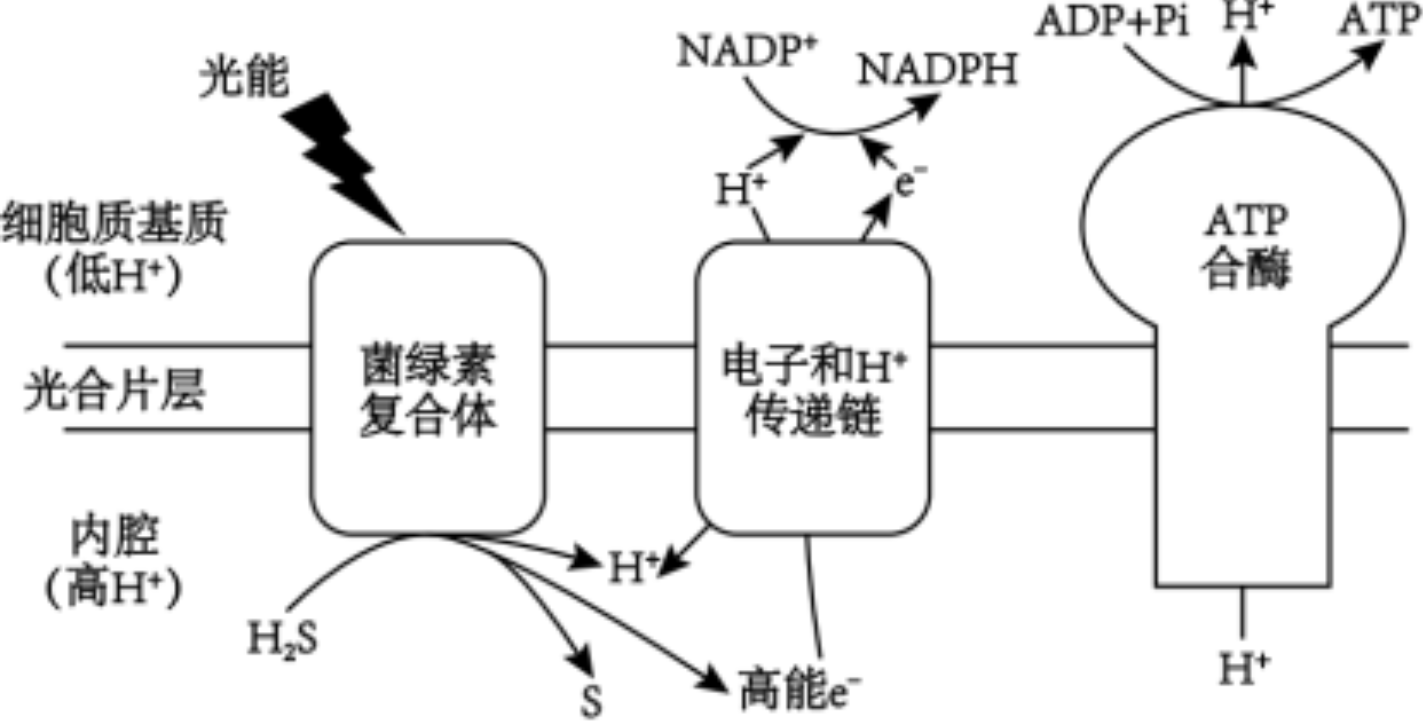
\includegraphics[width=0.4\textwidth]{assists/14-2.jpg}
    \end{figure}
    \begin{adjustwidth}{2em}{}
        \begin{asparaenum}[A. ]
            \item 绿硫细菌产生的高能$e^-$长期储存在 NADPH中
            \item 叶绿体中的菌绿素复合体,用于吸收、传递、转化光能
            \item 绿硫细菌在光反应中,$\ce{H2S}$是电子供体
            \item $\ce{H+}$进入内腔需要的能量直接来自 $\ce{H2S}$分解时产生的能量
        \end{asparaenum}
    \end{adjustwidth}
    \begin{answer}
        C
    \end{answer}
    \begin{point}
        不产氧光合作用、光合作用中的电子转移与ATP合成
    \end{point}
    \begin{explanation}
        NADPH高度活泼,不能长期储存电子,NADPH最终将高能电子用于还原反向三羧酸循环的中间产物,C选项错误;绿硫细菌是原核生物,没有除核糖体以外的细胞器,B选项错误;S化合价$-2 \rightarrow 0$,提供了电子,A选项正确;$\ce{H+}$进入内腔需要的能量直接来自两侧$e^-$浓度差,D选项错误。
    \end{explanation}
\end{exercise}

\begin{exercise}
    研究发现,生物膜融合存在以下机制:不同生物膜上的蛋白质相互作用形成螺旋状的复合蛋白,使磷脂分子失去稳定进而重排形成融合孔,最后实现生物膜的相互融合,过程如图所示。下列叙述错误的是\quad(\quad)
    \begin{figure}[h!]
        \centering
        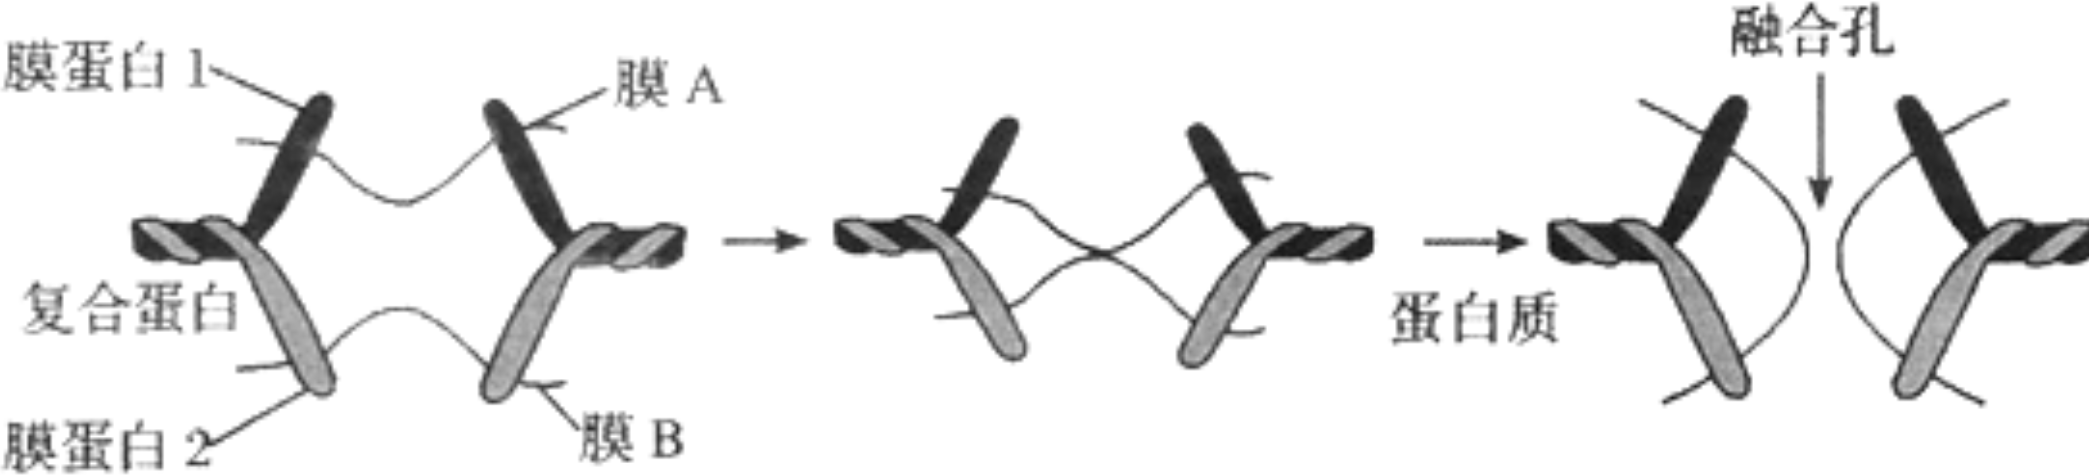
\includegraphics[width=0.6\textwidth]{assists/12-1.jpg}
    \end{figure}
    \begin{adjustwidth}{2em}{}
        \begin{asparaenum}[A. ]
            \item 膜蛋白1、2形成螺旋状结构涉及自身构象的变化
            \item 自然界中正常情况下,膜蛋白1、2都来自同一个生物体
            \item 胰岛素或乙酰胆碱可通过囊泡与细胞膜融合释放,从而传递信息
            \item 细胞膜的融合有一定特异性
        \end{asparaenum}
    \end{adjustwidth}
    \begin{answer}
        B
    \end{answer}
    \begin{point}
        流动镶嵌模型
    \end{point}
    \begin{explanation}
        自然界中,膜蛋白1、2不一定来自同一生物体,如精卵结合时,B选项错误。
    \end{explanation}
\end{exercise}
\begin{exercise}
    泛素化是指泛素分子(一类低分子量的蛋白质)在一系列酶的作用下,将细胞内的蛋白质分类,从中选出靶蛋白分子,并对靶蛋白进行特异性修饰的过程。最新研究表明,核蛋白UHRF1在有丝分裂中催化驱动蛋白EG5泛素化,进而调控细胞周期转换与细胞增殖,该研究揭示了UHRF1调控有丝分裂纺锤体结构和染色体行为的新机制,如图所示。下列相关叙述错误的是\quad(\quad)\vspace{-2em}
    \begin{figure}[h!]
        \centering
        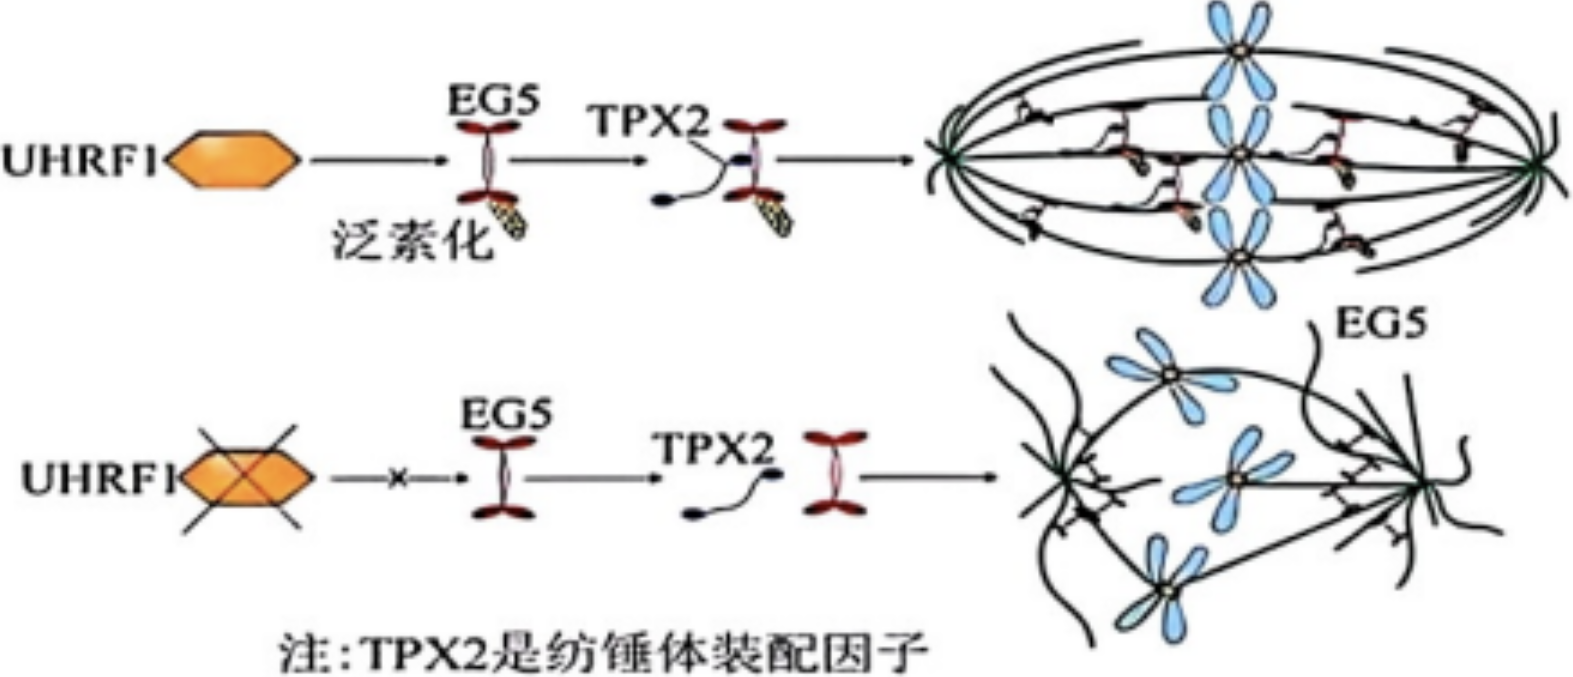
\includegraphics[width=0.5\textwidth]{assists/14-1.jpg}
    \end{figure}
    \begin{adjustwidth}{2em}{}
        \begin{asparaenum}[A. ]
            \item TPX2确保有丝分裂中期EG5在纺锤丝上的正确分布
            \item 在敲除TPX2的细胞中EG5则不能结合到纺锤丝上
            \item UHRF1蛋白缺失会导致染色体无法形成纺锤体,致使有丝分裂过程受阻
            \item 该研究为UHRF1作为潜在抗癌药物靶点提供理论依据
        \end{asparaenum}
    \end{adjustwidth}
    \begin{answer}
        B
    \end{answer}
    \begin{point}
        纺锤体的形成、流程图
    \end{point}
    \begin{explanation}
        由图可知,在敲除UHRF1的细胞中EG5不能与TPX2结合,但EG5最终还是结合在纺锤丝上,所以可以推断,当敲除TPX2时,EG5仍能结合在纺锤丝上,B选项错误。
    \end{explanation}
\end{exercise}

\begin{exercise}
    砷可严重影响植物的生长发育。拟南芥对砷胁迫具有一定的耐受性,为探究其机制,研究者进行了相关实验。回答下列问题:

    (1) 砷通过转运蛋白F进入根细胞时需消耗能量,该运输方式属于 \blank。砷的累积可导致细胞内自由基含量升高,自由基造成细胞损伤甚至死亡的原因为 \blank(答出两点即可)。

    \begin{answer}
        主动运输\qquad 损伤生物膜、引起基因突变、使蛋白质活性下降\chdots
    \end{answer}
    \begin{point}
        物质运输、细胞衰老——自由基学说
    \end{point}
    \begin{explanation}
        \fs{略}
    \end{explanation}

    \begin{figure}[h!]
        \flushright
        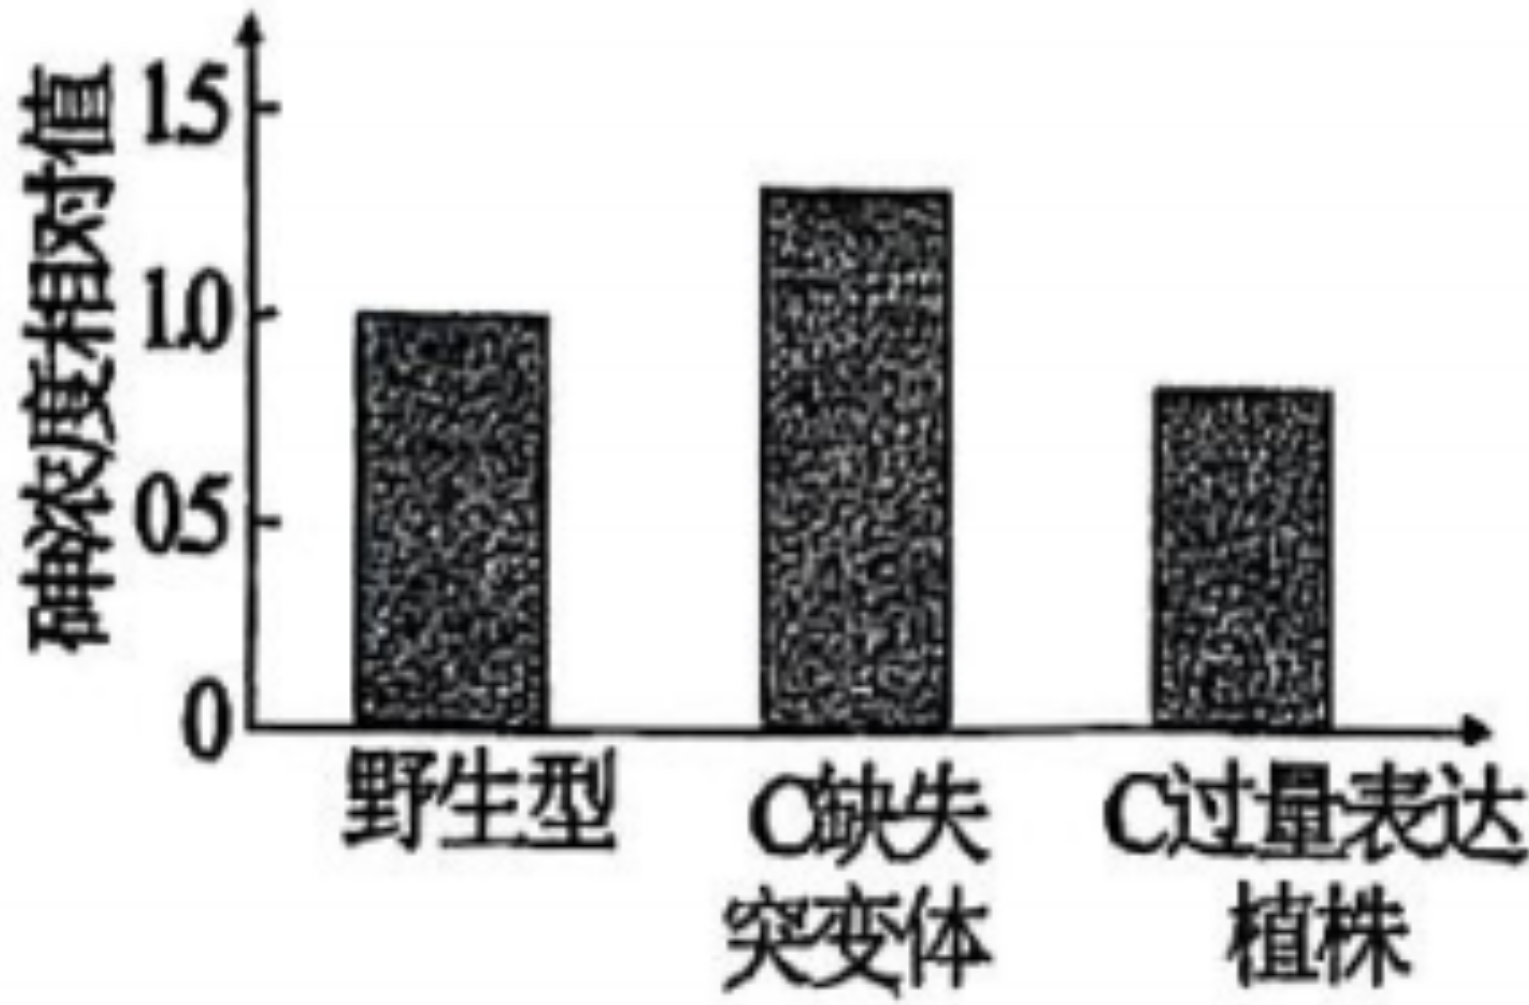
\includegraphics[width=0.3\textwidth]{assists/d1-1.jpg}

    \end{figure}

    \begin{adjustwidth}{}{0.32\textwidth}\vspace{-13em}

        \textcolor{white}{spa}(2)针对砷吸收相关基因C缺失和过量表达的拟南芥,研究者检测了其根细胞中砷的含量,结果如图。
        由此推测,蛋白C可 \blank 根对砷的吸收。进一步研究表明,砷激活的蛋白C可使F磷酸化,磷酸化的F诱导细胞膜内陷,形成含有蛋白F的囊泡。由此判断,激活的蛋白C可使细胞膜上转运蛋白F的数量 \blank,造成根对砷吸收量的改变。囊泡的形成过程体现了细胞膜在结构上具有 \blank 的特点。
    \end{adjustwidth}
    \begin{answer}
        抑制\qquad 减少\qquad 流动性
    \end{answer}
    \begin{point}
        数据分析、生物膜的结构特点
    \end{point}
    \begin{explanation}
        C缺失突变体的砷浓度相对值较高,C过量表达突变体的砷浓度相对值较低,推测蛋白C可抑制对砷的吸收;带有转运蛋白F的“细胞膜内陷”,减少了细胞膜上转运蛋白F的数量;\fs{略}
    \end{explanation}

    (3) 砷和磷可竞争性通过转运蛋白F进入细胞。推测在砷胁迫下植物对磷的吸收量 \blank,结合(2)和(3)的信息,分析其原因:\blank(答出两点即可)。

    \begin{answer}
        降低\qquad 砷胁迫下,细胞膜上转运蛋白F的数量减少、砷和磷竞争性通过转运蛋白F进入细胞、砷胁迫下,与磷结合的转运蛋白F数量减少,导致植物对磷的吸收量减少(或其他合理答案)
    \end{answer}
    \begin{point}
        竞争性抑制
    \end{point}
    \begin{explanation}
        \fs{略}
    \end{explanation}

\end{exercise}

\begin{exercise}
    研究者用荧光染料对细胞膜上某些分子进行处理,使膜发出荧光后,再用高强度激光照射细胞膜某区域。发现该区域瞬间被“漂白”(荧光消失)一段时间后,该漂白区域荧光逐渐恢复(如图甲)。图乙是该区域荧光强度随时间的变化而得到的荧光漂白恢复曲线。

    \begin{figure}[h!]
        \centering
        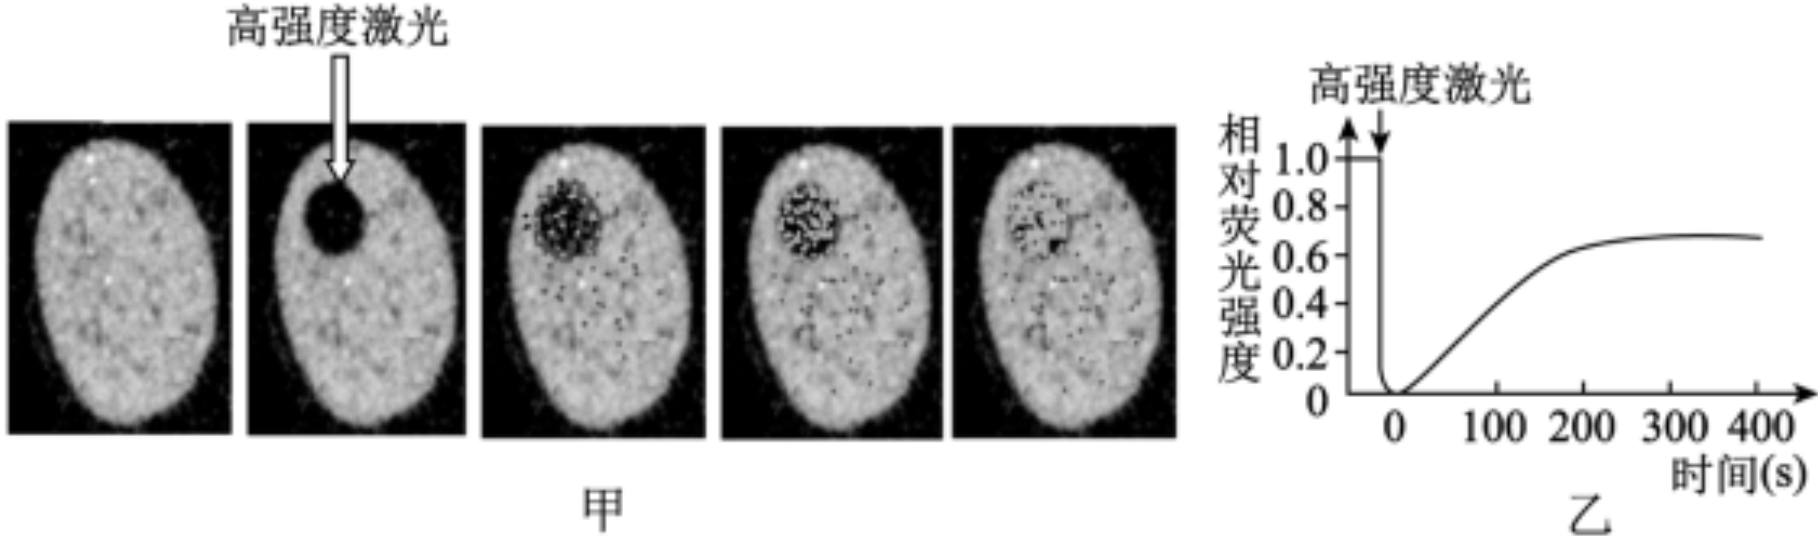
\includegraphics[width=0.8\textwidth]{assists/d2-1.jpg}
    \end{figure}

    (1)细胞膜的组成元素一定含有\blank,细胞膜主要由\blank 组成,此外还含有\blank。根据课本中人鼠细胞融合实验可知,荧光染料通常标记的是细胞膜上的\blank(填一种化合物)。

    \begin{answer}
        C、H、O、N、P \qquad 脂质和蛋白质 \qquad 糖类 \qquad 蛋白质
    \end{answer}
    \begin{point}
        细胞膜的组成、荧光标记法
    \end{point}
    \begin{explanation}
        \fs{略}
    \end{explanation}

    (2)细胞膜上被漂白区域的荧光得以恢复,推测其可能的原因:\circled{1}被漂白区域内细胞膜成分分子带有的荧光染料的荧光会自行恢复;\circled{2}\blank。

    \begin{answer}
        被漂白区域内外的细胞膜成分分子在流动
    \end{answer}
    \begin{point}
        荧光标记的人鼠细胞融合实验
    \end{point}
    \begin{explanation}
        \fs{略}
    \end{explanation}

    (3)研究发现,如果用特定方法去除细胞膜中的胆固醇,使膜结构上蛋白质分子停泊的“平台”被拆解,漂白区域荧光恢复所需的时间\blank,说明胆固醇对组成细胞膜成分分子的运动具有\blank 作用,该结果\blank(填“支持”或“不支持”)推测\circled{2}。此项研究体现了细胞膜的\blank(“结构”或“功能”)特性。

    \begin{answer}
        缩短\qquad 抑制\qquad 支持\qquad 结构
    \end{answer}
    \begin{point}
        胆固醇对于细胞膜流动性的影响、细胞膜的结构特性
    \end{point}
    \begin{explanation}
        用特定方法去除细胞膜中的胆固醇,会导致膜结构上蛋白质分子停泊的“平合“拆解,进而解除胆固醇的抑制作用,使蛋白质分子运动速率加快,漂白区域荧光恢复的时间缩短,且能说明荧光的恢复是漂白区域内外细胞膜成分分子相互运动的结果,结果支持推测\circled{2}。细胞膜成分分子的运动使荧光恢复,说明了细胞膜具有一定的流动性,这是细胞膜的结构特点。
    \end{explanation}
\end{exercise}
\begin{exercise}

    当光照过强,积累的NADPH会造成叶绿体损伤,导致光合速率下降。如图表示eATP与呼吸链对某植物光合作用的影响(细胞内ATP为iATP,细胞外ATP为eATP),由交替氧化酶(AO)主导的呼吸途径利于植物抵抗强光。

    \begin{figure}[h!]
        \centering
        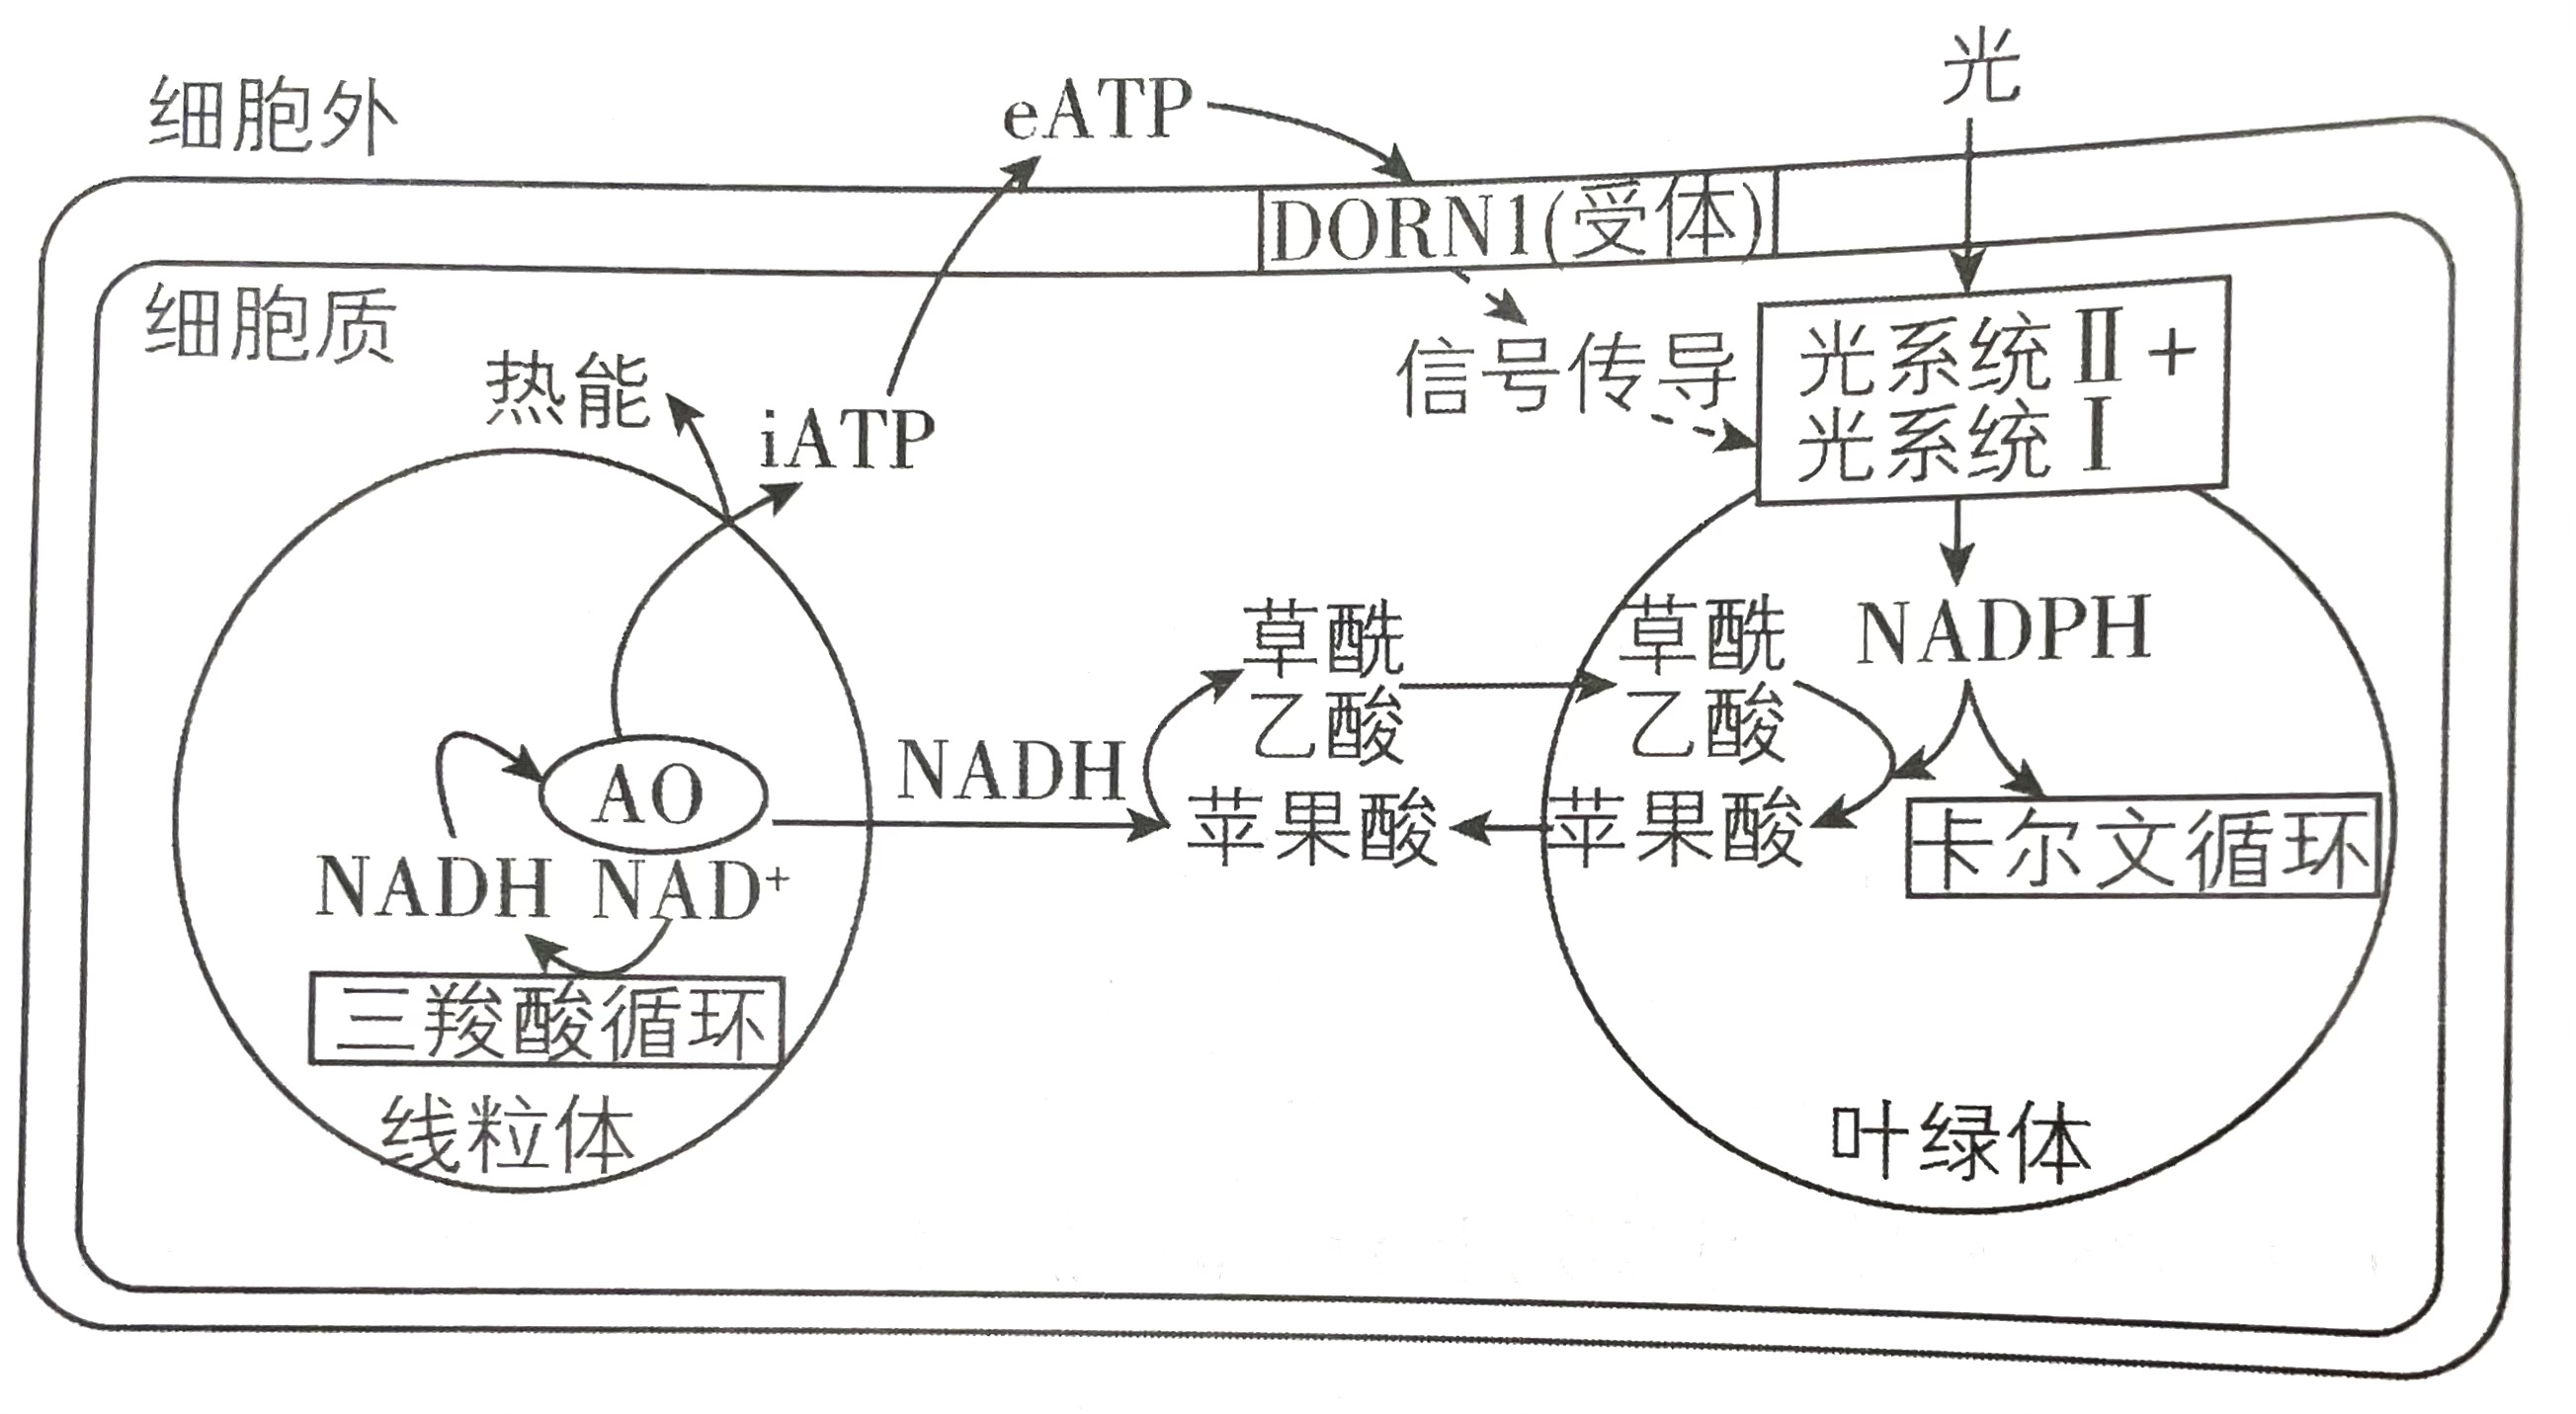
\includegraphics[width=0.5\textwidth]{assists/19-1.jpg}
    \end{figure}
    \noindent 根据所学知识回答下列问题:

    (1)产生iATP的场所有\blank(至少写出两点)。

    \begin{answer}
        线粒体、细胞质基质、叶绿体(类囊体)
    \end{answer}
    \begin{point}
        ATP的胞内合成
    \end{point}
    \begin{explanation}
        \fs{略}
    \end{explanation}


    (2)光系统\Romannumeral{1}和光系统\Romannumeral{2}是由蛋白质和光合色素组成的复合物,其作用是\blank。

    \begin{answer}
        实现对光能的吸收、传递、转化;产生ATP和NADPH供暗反应使用;进行水的光解
    \end{answer}
    \begin{point}
        光合反应的作用
    \end{point}
    \begin{explanation}
        \fs{略}
    \end{explanation}

    (3) 氰化物可抑制细胞色素氧化酶的活性从而抑制细胞呼吸,植物可通过AO进行抗氰呼吸,但该过程释放的热能更多。与正常细胞呼吸相比,抗氰呼吸过程中生成的ATP\blank(填"较多"或"较少")。

    \begin{answer}
        较少
    \end{answer}
    \begin{point}
        呼吸作用的影响因素
    \end{point}
    \begin{explanation}
        通过AO进行的抗氰呼吸过程释放的热量更多,说明其呼吸作用过程中释放出的能量以热能形式散失的比例更高,因为存在能量守恒,故抗氰呼吸过程中生成的 ATP 较正常细胞呼吸少。
    \end{explanation}

    (4)交替氧化酶(AO)主导的呼吸途径利于植物抵抗强光的原因是\blank。

    \begin{answer}
        AO消耗NADH,有利于促进草酰乙酸和苹果酸循环,加速NADPH的利用,减少其对叶绿体的损伤
    \end{answer}
    \begin{point}
        阅读理解、光反应的影响因素
    \end{point}
    \begin{explanation}
        由题干“当光照过强,积累的NADPH会造成叶绿体损伤,导致光合速率下降”以及题图中的信息可知,交替氧化酶(AO)主导的呼吸途径利于植物抵抗强光的原因是该途径可以消耗更多的 NADH,有利于促进草酰乙酸和苹果酸循环,加速 NADPH的利用,使 NADPH 更多地转化为 $\ce{NADP+}$,从而减少 NADPH 的积累,降低强光对叶绿体的损伤。
    \end{explanation}

    (5)研究者推测,eATP可能是作为\blank 调节植物的光合作用。为探究强光条件下eATP对植物光合速率的影响,请写出实验思路\blank。

    \begin{answer}
        信号分子\qquad 生长状况相同的若干植物,平均分成两组,分别标记为A组和B组。将A组植物置于强光条件下,同时向其喷施适量的eATP 溶液;将B组植物置于相同的强光条件下,喷施等量的蒸馏水作为对照。在其他条件相同且适宜的环境中培养一段时间后,分别测定两组植物的光合速率(或用正常植物和DORN1缺陷型植物作对照,在强光条件下,测定两组植物的光合速率)
    \end{answer}
    \begin{point}
        阅读理解、实验设计
    \end{point}
    \begin{explanation}
        研究者推测,eATP 可能作为信号分子调节植物的光合作用。
        为探究强光条件下 eATP 对植物光合速率的影响,实验思路为将生长状况相同的若干植物,平均分成两组,分别标记为A组和B组。将A组植物置于强光条件下,同时向其喷施适量的eATP 溶液;将B组植物置于相同的强光条件下,喷施等量的蒸馏水作为对照。在其他条件相同且适宜的环境中培养一段时间后,分别测定两组植物的光合速率。

    \end{explanation}

\end{exercise}
\begin{exercise}
    学习以下材料,回答(1)$\sim$(5)题。
    \begin{center}\vspace{-1em}
        \hei{LBR蛋白在有丝分裂中的作用}
    \end{center}\vspace{-0.5em}
    {\kaishu

    在有丝分裂过程中,内质网与线粒体之间的接触位点(ERM)数量显著增加。研究发现,跨膜蛋白LBR可与特定蛋白质互作,形成特异性的ERM。它的缺失会导致细胞分裂的延迟甚至失败。

    为探究LBR在有丝分裂过程中的作用,研究人员制备了敲除LBR基因的肿瘤细胞(KO),与正常肿瘤细胞(WT)进行对比实验,统计分裂间期和分裂期的细胞占比,结果如图1。进一步观察线粒体和内质网的亚显微结构,发现KO组细胞中ERM减少,如图2。此外,在细胞分裂的不同阶段,ATP的产生量存在显著差异。

    内质网是真核生物中的钙库之一,在$\ce{Ca^2+}$的储存和释放中起重要作用。有丝分裂过程中,中期细胞的线粒体$\ce{Ca^2+}$内流激增,促进了ATP的产生。充足的能量供应对于中期向后期的过渡和细胞分裂的完成至关重要。这项研究为细胞周期相关疾病的治疗提供了新的视角。
    }
    \begin{figure}[h!]
        \centering
        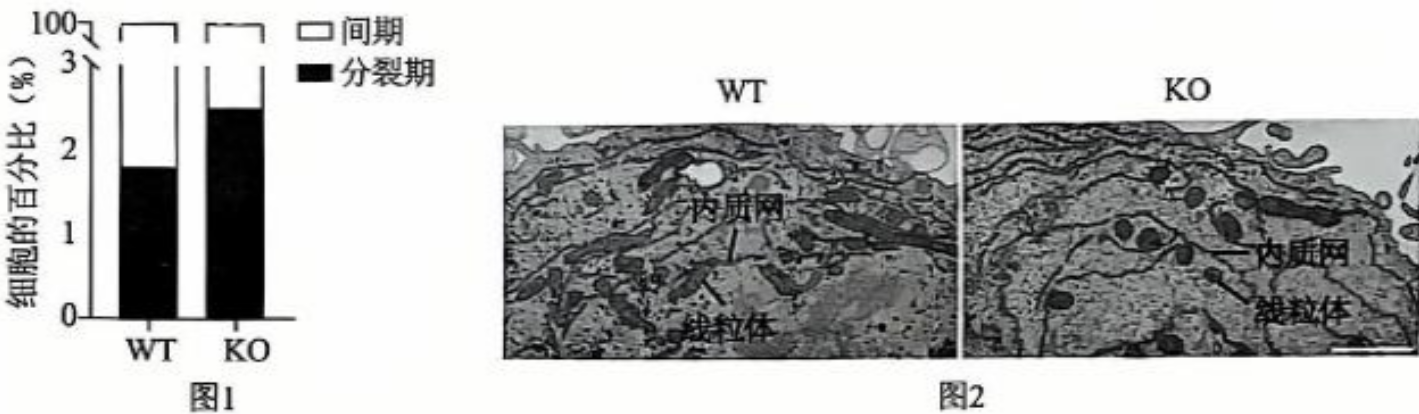
\includegraphics[width=0.6\textwidth]{assists/17-1.jpg}
    \end{figure}\vspace{-1em}

    (1)细胞有丝分裂中期染色体排列在细胞中央\blank 位置,后期细胞中的染色体在\blank 的牵引下向两极移动。

    \begin{answer}
        赤道板\qquad 纺锤丝
    \end{answer}
    \begin{point}
        有丝分裂染色体行为
    \end{point}
    \begin{explanation}
        \fs{略}
    \end{explanation}

    (2)图1结果说明\blank 。为进一步确定LBR作用的具体时期,用药物对细胞进行同步化处理。若\blank ,则说明LBR作用于中期向后期的过渡时期。

    \begin{answer}
        缺失LBR蛋白,细胞周期被阻断在分裂期\qquad 与WT相比,KO组中期细胞占比高,后期细胞占比低
    \end{answer}
    \begin{point}
        数据分析、阅读理解
    \end{point}
    \begin{explanation}
        题图中可知 KO组间期细胞百分比降低而分裂期细胞百分比升高,说明缺失 LBR 蛋白,细胞周期被阻断在分裂期;根据有丝分裂中期和后期的特点可知,为进一步确定LBR作用的具体时期,用药物对细胞进行同步化处理。若与WT组相比,KO组中期细胞占比高,后期细胞占比低,则说明 LBR 作用于中期向后期的过渡时期。
    \end{explanation}

    (3)根据文章内容,完善LBR的作用机制:LBR与特定分子结合$\rightarrow$ \blank $\rightarrow$ $\ce{Ca^2+}$ 由 \blank 进入\blank $\rightarrow$ ATP合成,细胞分裂进入后期。

    \begin{answer}
        形成特异性ERM \qquad 内质网 \qquad 线粒体
    \end{answer}
    \begin{point}
        阅读理解
    \end{point}
    \begin{explanation}
        由题图可知,在有丝分裂过程中,内质网与线粒体之间的接触位点(ERM)数量显著增加;跨膜蛋白LBR 可与特定蛋白质互作,形成特异性的 ERM;内质网是真核生物中的钙库之一;有丝分裂过程中,中期细胞的线粒体 $\ce{Ca^2+}$内流激增,促进了ATP的产生;充足的能量供应对于中期向后期的过渡和细胞分裂的完成至关重要;通过分析可知,LBR 的作用机制为 LBR 与特定分子结合一形成特异性 ERM一$\ce{Ca^2+}$由内质网进入线粒体一ATP合成,细胞分裂进入后期。
    \end{explanation}

    (4)请解释足量ATP对于中期向后期过渡至关重要的原因。

    \begin{answer}
        着丝粒分裂、姐妹染色单体分开,向两级移动需要大量能量,消耗足量ATP
    \end{answer}
    \begin{point}
        有丝分裂中后期的物质与能量变化
    \end{point}
    \begin{explanation}
        ATP 是细胞生命活动的直接能源物质,足量ATP 对于中期向后期过渡至关重要的原因是着丝粒的分裂、纺锤丝牵引染色体向两极移动需要消耗 ATP。
    \end{explanation}

    (5)本研究为肿瘤治疗提供了哪些思路?

    \begin{answer}
        研制抑制LBR作用的药物,将肿瘤细胞的细胞周期阻断
    \end{answer}
    \begin{point}
        阅读理解
    \end{point}
    \begin{explanation}
        由题干信息可知,敲除LBR 基因的肿瘤细胞(KO),与正常肿瘤细胞(WT)进行对比实验,统计分裂间期和分裂期的细胞占比,结果说明缺失 LBR 蛋白,细胞周期被阻断在分裂期;由此可知,可以通过研制阻断LBR 作用的药物为肿瘤治疗提供新思路。
    \end{explanation}
\end{exercise}
\end{document}